\documentclass{report}

\usepackage{fullpage}
\usepackage[skip=4pt]{caption} % ``skip'' sets the spacing between the figure and the caption.
\usepackage{tikz}
\usepackage{pgfplots}   % Needed for plotting
\pgfplotsset{compat=newest}
\usepgfplotslibrary{fillbetween}  % Allow for highlighting under a curve
\usepackage{amsmath}    % Allows for piecewise functions using the ``cases'' construct
%\usepackage{mathrsfs}   % Use the ``\mathscr'' command in an equation.

\usepackage[obeyspaces,spaces]{url} % Used for typesetting with the ``path'' command
\usepackage[hidelinks]{hyperref}   % Make the cross references clickable hyperlinks
\usepackage[bottom]{footmisc} % Prevents the table going below the footnote
\usepackage{nccmath}    % Needed in the workaround for the ``aligncustom'' environment
\usepackage{amssymb}    % Used for black QED symbol   
\usepackage{bm}    % Allows for bolding math symbols.
\usepackage{tabto}     % Allows to tab to certain point on a line
\usepackage{float}

\newcommand{\hangindentdistance}{1cm}
\setlength{\parindent}{0pt}
\setlength{\leftskip}{\hangindentdistance}
\setlength{\hangafter}{1}
\setlength{\parskip}{1em}


% Set up page formatting
\usepackage{todonotes}
\usepackage{fancyhdr} % Used for every page footer and title.
\pagestyle{fancy}
\fancyhf{} % Clears both the header and footer
\renewcommand{\headrulewidth}{0pt} % Eliminates line at the top of the page.
\fancyfoot[LO]{CMPS218 \textendash\ Homework \#1} % Left
\fancyfoot[CO]{\thepage} % Center
\fancyfoot[RO]{Zayd Hammoudeh} %Right

% Change interline spacing.
\renewcommand{\baselinestretch}{1.1}
\newenvironment{aligncustom}
{ \csname align*\endcsname % Need to do this instead of \begin{align*} because of LaTeX bug.
    \centering
}
{
  \csname endalign*\endcsname
}
%--------------------------------------------------


\title{\textbf{CMPS218 \textendash\ Homework \#1}}
\author{Zayd Hammoudeh}

%---------------------------------------------------%
% Define the Environments for the Problem Inclusion %
%---------------------------------------------------%
\newcounter{subProbCount}       % Initialize the subproblem counter
\newcounter{problemCount}
\setcounter{problemCount}{0} % Reset the subproblem counter
\newenvironment{problemshell}{
  \par%
  \medskip
  \leftskip=0pt\rightskip=0pt%
}
{
  \par\medskip
  \setcounter{subProbCount}{1} % Reset the subproblem counter
}
\newenvironment{problem}[3]
{%
  \begin{problemshell}
    \noindent \textit{Chapter \##1.#2, Problem \##3} \\
    \bfseries
}
{
  \end{problemshell}
}
\newenvironment{subproblem}
{%
  \par%
  \medskip
  \leftskip=0pt\rightskip=0pt%
  \bfseries
  % Print the subproblem count and offset to the left
  (\alph{subProbCount}) \hangindent=\hangindentdistance \hangafter=1 \tabto{\hangindentdistance}
}
{
  \stepcounter{subProbCount} % Increment the subproblem counter
  \par\medskip
}
\newcommand{\problemspace}{\\[0.4em]}

\begin{document}
  \maketitle
  
  \begin{problem}{2}{9}{33}
    Two points are selected at random on a straight line segment of length~1.  What is the probability that a triangle can be constructed out of the three resulting segments.
  \end{problem}
  
  For the two randomly selected points,~$x_1$ and $x_2$, define $L_{\max}$ as the length of the longest segment.  By the triangle inequality theorem, it is clear that a triangle can only be formed from these three segments if ${L_{\max} < 0.5}$.  
  
  
  Consider the tuple ${(x_1,x_2)}$. Each point in the domain $(0,1)^2$ is equally likely since the points are selected randomly.  Figure~\ref{fig:problem2.9.33} shows the portions of this domain (highlighted in light blue) where the lines segments induced by $x_1$ and $x_2$ can be used to form a triangle.
  
  \begin{figure}[h]
    \centering
    \scalebox{0.6}{ % Scaling factor for the plot.
      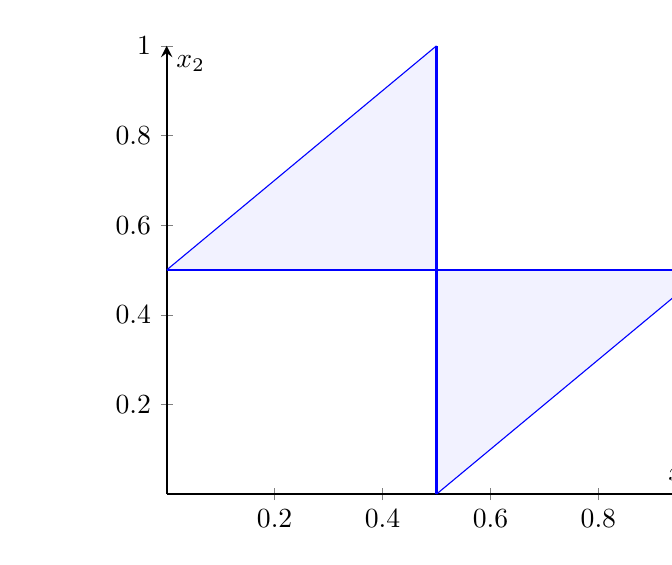
\begin{tikzpicture}
      \begin{axis}[ 
        axis line style = thick,
        axis lines=middle,
        xmin=0,
        xmax=1,
        ymin=0,
        ymax=1,
        xlabel=$x_1$,
        ylabel={$x_2$},
      ] 
      \addplot[name path=half, smooth, color=blue, domain=0:1] {0.5};
      \addplot[name path=f_1, smooth, color=blue, domain=0:0.5] {0.5 + x};
      \addplot[name path=f_2, smooth, color=blue, domain=0.5:1] {-.5+x};
      \draw [color=blue, thick] (0.5,0) -- (0.5,1);
      \path[name path=axis] (axis cs:0,0) -- (axis cs:1,0); % X axis for fill between
      \addplot [
        thick,
        color=blue,
        fill=blue, 
        fill opacity=0.05
        ] 
        fill between[
        of=f_1 and half,
        soft clip={domain=0:.5},
      ];
      \addplot [
        thick,
        color=blue,
        fill=blue, 
        fill opacity=0.05
        ] 
        fill between[
        of=f_2 and half,
        soft clip={domain=0.5:1},
      ];
      \end{axis}
      \end{tikzpicture}
    }
    \caption{Regions of the domain where the line segments induced by $(x_1,x_2)$ form a triangle.}\label{fig:problem2.9.33}
  \end{figure}

  Since the probability selecting any point within the above domain is uniform, the probability of selecting points that form a triangle is found via:
  
  \begin{aligncustom}
    \Pr(\text{Form a line}) &= \frac{2 * \text{Area of Trianges}}{\text{Total Area}}\\
                            &= \frac{2 * \left(\frac{1}{2}\right)^{2}}{1}\\
                            &= \boxed{\frac{1}{4}}
  \end{aligncustom}
  
  \newpage
  \begin{problem}{5}{9}{30}
    \textit{Scientific American} carried the following puzzle in 1975.
    \problemspace
    \textbf{The poisoned glass:} \textnormal{\textit{'Mathematicians are curious birds,' the police commissioner said to his wife. 'You see, we had all those partly filled glasses lined up in rows on a table in the hotel kitchen. Only one contained poison, and we wanted to know which one before searching the glass for fingerprints.  Our lab could test the liquid in each glass, but the tests take time and money, so we wanted to make as few of them as possible by simultaneously testing mixtures of small samples from groups of glasses.  The university sent over a mathematics professor to help us.  He counted the glasses, smiled and said: \\ ``Pick any glass you want, Commissioner. We'll test it first.'' \\ ``But won't that waste a test?'' I asked. \\ ``No,'' he said. ``it's part of the best procedure.  We can test one glass first.  It doesn't matter which one.'' \\ `How many glasses were there to start with?' the commissioner's wife asked. \\ 'I don't remember. Somewhere between 100 and 200.'} \\What was the exact number of glasses?}
    \problemspace
    Solve this puzzle and then explain why the professor is in fact wrong and the commissioner was right.  What is in fact the optimal procedure for identifying the one poisoned glass?  What is the expected waste relative to this optimum if one followed the professor's strategy?  Explain the relationship to symbol coding.
  \end{problem}

  The test for poison has a binary outcome, i.e.,~the sample either has poison or not.  Therefore, assuming each cup has poison with equal probability, the size of the remaining set of glasses is, on average, cut in half with each test.
  
  If the number of glasses,~$n$, is a power of~$2$, then the number of tests required is $\lg n$, where $\lg$ is the base-$2$ logarithm.  Note that the only power of~2 between 100 and 200 is 128.  There was one extra glass that the professor tested separately.  Therefore, there was \boxed{129~\text{glasses}}.
  
  \begin{table}[h]
    \centering
    \begin{tabular}{c|c|c}
      \hline
      Glass ID & Probability of Poison & \# Tests  \\\hline
      1        & 1/129                 & 1         \\\hline
      2-129    & 128/129               & 1 + 7 = 8 \\\hline
    \end{tabular}
    \caption{Number of tests required using the professors strategy}\label{tab:problem5.9.20-Prof}
  \end{table}
  
  Table~\ref{tab:problem5.9.20-Prof} shows the number of tests required when using the professors strategy.  Glass~\#1 represents the first glass test.  In the unlikely event that glass has the poison, no additional testing is required. In contrast, the poison is in one of the other 128~glasses, seven tests (plus the additional one for the first glass) are required.  Using this strategy, the expected number of tests is:
  
  \begin{aligncustom}
    \mathbb{E}(\text{Professor's Strategy}) &= \frac{1}{129} \cdot 1 + \frac{128}{129} \cdot 8 \\
                                            &\approx \boxed{7.946}\text{.} 
  \end{aligncustom}
  
  \begin{table}[h]
    \centering
    \begin{tabular}{c|c|c}
      \hline
      Glass ID & Probability of Poison & \# Tests  \\\hline
      1        & 1/129                 & 7 + 1     \\\hline
      2-129    & 128/129               & 7         \\\hline
    \end{tabular}
    \caption{Number of tests required using the optimum strategy}\label{tab:problem5.9.20-Opt}
  \end{table}
  
  Rather than testing the one additional glass separately as the professor did, the optimum approach would be to test that glass last since it is very unlikely to have the poison.  Table~\ref{tab:problem5.9.20-Opt} shows the number of tests required using this optimum strategy.    Using this optimum strategy, the expected number of tests is:
 
  
  \begin{aligncustom}
    \mathbb{E}(\text{Optimum Strategy}) &= \frac{1}{129} \cdot 8 + \frac{128}{129} \cdot 7 \\
    &\approx \boxed{7.008}\text{.} 
  \end{aligncustom}
  
  It is clear then that the expected waste is \boxed{0.938}.

  {\color{red} EXPLAIN WHY LIKE SYMBOL CODES}

  \newpage
  \begin{problem}{20}{2}{2}
    Show that as the stiffness~$\beta$ goes to~$\infty$, the soft K-means algorithm becomes identical to the original hard K-means algorithm except for the way in which means assigned no points behave.  Describe what those means do instead of sitting still.
  \end{problem}

  In the standard or ``hard'' K-means algorithm, each point is assigned to exactly one cluster.  As such, each of a cluster's points have equal membership.
  
  Soft K-means reduces the rigidity of the standard K-means by introducing a new ``stiffness'' hyperparameter,~$\beta$.  Rather than each point being a member of exclusively one cluster, the \textit{responsibility} for that point is shared among all $K$~clusters.  For a cluster~$k$ and point~$\textbf{x}^{(n)}$, the responsibility,~$r_{k}^{(n)}$ is: 
  
  \begin{equation}
    r_k^{(n)} = \frac{\exp(-\beta d(\textbf{m}^{k'}, \textbf{x}^{(n)}))}{\sum_{k} \exp(-\beta d(\textbf{m}^{k'}, \textbf{x}^{(n)}))}
  \end{equation}
  
  \noindent
  where $d$ is the distance metric, and $m^{k}$ is the center of cluster~$k$.
  
  As $\beta$ increases, then even small differences in $d$ will cause massive disparities in responsibility.  As $\beta$ approaches infinity, all responsibility for a point will be assigned to its nearest cluster.  This behavior is exactly the same as standard, ``hard'' K-means.
  
  When performing Soft K-means with $\beta \rightarrow \infty$, it is possible that some clusters may have no responsibility for no points.  In which case, the centroid approaches the zero vector.
  
  
\end{document}

